% classes
\documentclass{article}

% packages
\usepackage{graphicx}
\usepackage{fancyhdr} % Required for custom headers
\usepackage{lastpage} % Required to determine the last page for the footer
\usepackage{extramarks} % Required for headers and footers
\usepackage{courier} % Required for the courier font

\usepackage{color}
\usepackage{enumitem}

\usepackage{hyperref}


% page layout

\topmargin=-0.45in
\evensidemargin=0in
\oddsidemargin=0in

\textwidth=6.5in
\textheight=9.0in

\headsep=0.25in

\linespread{1.1} % Line spacing
 
\pagestyle{fancy}

% headers and footers

\fancyhf{}

\lhead{INTR 100 Breaking Intuition}

\rhead{
\includegraphics[width=0.045\textwidth]{wmlogo.jpg}}



% document body

\begin{document}

\vspace*{.01mm}

\begin{center}

\Large{\textcolor{blue}{\textbf{Lab 2.}  Data Science Basics: Packages, Datasets and Spatial Objects}}

\vspace{4mm}

\textit{Due by noon on Friday, September 11th}\\

\end{center}

\begin{figure}[h!]
\begin{center}
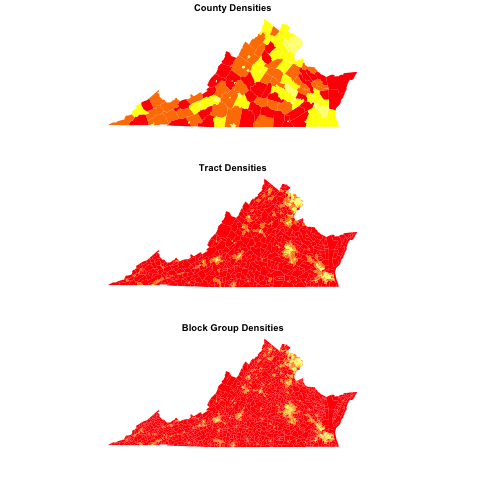
\includegraphics[width=0.9\textwidth]{virginia.png}

\end{center}
\end{figure}

\setlength{\parindent}{0cm}

\large{\textit{"Everything is related to everything else, but near things are more related than distant things."}
\begin{flushright}
Tobler, 1970
\end{flushright}
}


\newpage

% Enumerate the Laboratory Objectives

\large{\textbf{Laboratory in Brief:}}

\vspace{4mm}

\setlength{\leftskip}{1cm}

\setlength{\parindent}{0cm}

The purpose of this laboratory is to introduce students to working with spatial data by statistically describing it and quantitatively analysing it in an increasingly disaggregate manner.  You will be introduced to the statistical programming framework R, by learning how to install a package and execute some of its basic functions.  Initially you will use the chloropleth package to statistically describe a single demographic characteristic of one American state at the county level.  Following this, you will use the USCensus2010 package to create a spatial R object and increase the disaggregate level of analysis from county to sub-county areas.  Finally, you will learn how to remotely access the Census Bureau's Application Program Interface (API) directly from within R, create a sub-county area spatial object, and statistically describe that area by one or more demographic characteristics.

\vspace{4mm}

\setlength{\leftskip}{0cm}

\large{\textbf{Specific Objectives:}}

\begin{enumerate}[leftmargin=15mm]

\item To install the chloropleth package in R and create a map that statistically and spatially describes a demographic characteristic of one American State, county by county

\item To add a dataset, create a spatial object in R and create a map that statistically and spatially describes a demographic characteristic of several bordering counties within a state, tract by tract

\item To obtain data from the Census bureau Application Program Interface (API), create a R object and create a map that statistically and spatially describes a demographic characteristic of a county, block by block

\end{enumerate}

% Enumerate the Laboratory Objectives

\large{\textbf{Software and Resources you will need or will be helpful:}}

\begin{enumerate}[leftmargin=15mm]

\item The R Project for Statistical Computing otherwise known simply as R.  The R framework can be downloaded from \\ 
\url{https://www.r-project.org/}

\item Quick R, an online resource developed by Rob Kabacoff, a statistical consultant and methodologist, that is purposed towards introducing students to the power of R.  
\url{http://www.statmethods.net/}

\item Introduction to R, a pdf presentation created by Phil Spector, Applications Manager and Associate Adjunct Professor at Cal-Berkeley.  The pdf is more advanced than the the Quick-R online learning resource, but it covers many of R's basics with regard to functionality and emphasis on data management. \\ 
\url{https://www.stat.berkeley.edu/~spector/Rcourse.pdf}




\item Packages and datasets as instructed during the laboratory

\end{enumerate}


\newpage

\textbf{Grading}

\vspace{4mm}

\setlength{\leftskip}{1cm}

\setlength{\parindent}{0cm}

This lab will be graded in 4 parts.  \textbf{First}, you create a map that spatially describes your chosen state according some demographic characteristic, count by county (5\%).  \textbf{Second}, you will create a map that spatially describes two or more adjoining counties within your state according to some demographic characteristic, tract by tract (10\%).  \textbf{Third}, you will create a map that spatially describes a sub-county area of your state according to some demographic characteristic, block by block (15\%).  \textbf{Finally}, you will use each of these three maps in a report that spatially and statistically describes your state and its dissaggregate parts in accordance with one or more demographic or economic characteristics.  \\

Your lab report should include the following elements.

\begin{enumerate}[leftmargin=15mm]

\item all three maps, including description an analysis of each one

\item integrated into your report, a description of the code you used, in a manner that demonstrates your knowledge of how the code functioned and operated

\item an analysis of how increased disaggregation effects the statistical description of spatial data

\end{enumerate}

The highest grades will be reserved for work that not only spatially describes your chosen area in a statistically rigorous manner, but also uses quantitative analysis to suggest and support inferential conclusions. \\

\vspace{7mm}

\setlength{\leftskip}{0cm}

\large{\textit{"Data of geographic units are tied together, like bunches of grapes, not seperate, like balls in an urn.  Of course, mere contiguity in time and space does not of itself indicate independence between units in a relevant variable or attribute, but in dealing with social data, we know that by very virtue of their social character, persons, groups, and their characteristics are interrelated and not independent. Sampling error formulas may yet be developed which are applicable to these data, but until then, the older formulas must be used with great caution.  Likewise, other statistical measures must be carefully scrutinised when applied to these data"}
\begin{flushright}
Stephan, 1934
\end{flushright}
}

%----------------------------------------------------------------------------------------

\end{document}